%----------------------------------------------------------------------------------------
%	PACKAGES AND THEMES
%----------------------------------------------------------------------------------------
\documentclass[aspectratio=169,xcolor=dvipsnames]{beamer}
\usetheme{Simple}

\usepackage[brazil]{babel}
\usepackage{hyperref}
\usepackage{graphicx} % Allows including images
\usepackage{booktabs} % Allows the use of \toprule, \midrule and \bottomrule in tables
\usepackage{subcaption}

\addtobeamertemplate{frametitle continuation}{(}{)}

%----------------------------------------------------------------------------------------
%	TITLE PAGE
%----------------------------------------------------------------------------------------

% The title
\title[title]{Uma Implementação do Método FLIP para Simulação 2D de Fluidos}

\author[names] {Aluno: Gabriel Carvalho Sanches Rocha\newline{}Orientador: Paulo Aristarco Pagliosa}
\institute[FACOM] % Your institution may be shorthand to save space
{
    % Your institution for the title page
    Universidade Federal do Mato Grosso do Sul
    \vskip 3pt
}
\date{Março de 2021} % Date, can be changed to a custom date


%----------------------------------------------------------------------------------------
%	PRESENTATION SLIDES
%----------------------------------------------------------------------------------------

\begin{document}

\begin{frame}
    % Print the title page as the first slide
    \titlepage
\end{frame}

\begin{frame}{Roteiro}
    \tableofcontents
\end{frame}

%------------------------------------------------
\section{Introdução}
%------------------------------------------------

\begin{frame}{Introdução}
    \begin{itemize}[<+->]
        \item Animação baseada em física
        \item Simulação de fluidos
    \end{itemize}
\end{frame}

\begin{frame}{Introdução}
    \begin{itemize}[<+->]
        \item O que são fluidos?
        \item Como simular fluidos?
        \item Abordagens híbridas
        \begin{itemize}[<3->]
            \item \textit{Particle-in-cell}
            \item \textit{Fluid-implicit-particle}
        \end{itemize}
    \end{itemize}
    
    \only<1>
    {
        \begin{figure}
            \centering
            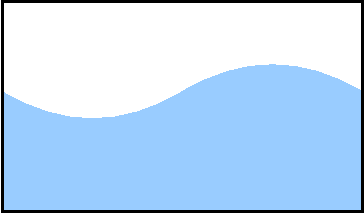
\includegraphics{figures/liquid.pdf}
            \caption{Líquido em um recipiente.}
            \label{fig:liquid}
        \end{figure}
    }
    
    \only<2>
    {
    \begin{figure}
        \begin{subfigure}{0.4\linewidth}
            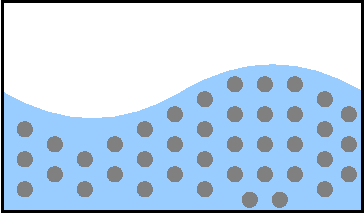
\includegraphics[width=\linewidth]{figures/LagrangianFramework.pdf}
            \caption{Líquido discretizado com partículas.}
        \end{subfigure}
        \begin{subfigure}{0.4\linewidth}
            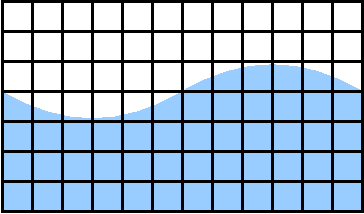
\includegraphics[width=\linewidth]{figures/EulerianFramework.pdf}
            \caption{Líquido discretizado com grade regular.}
        \end{subfigure}
        \centering
        \caption{Abordagens Lagrangiana e Euleriana.}
        \label{fig:frameworks}
    \end{figure}
    }
    
    \only<3>
    {
        \begin{figure}
            \centering
            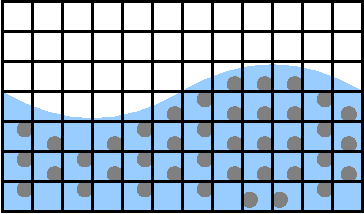
\includegraphics{figures/HybridFramework.pdf}
            \caption{Abordagem híbrida usando partículas e grade.}
            \label{fig:hybridframework}
        \end{figure}
    }
    
\end{frame}

\begin{frame}{Introdução}

\begin{itemize}
    \item Objetivos
    \begin{enumerate}
        \item Estudar os métodos híbridos PIC e FLIP
        \item Implementar os métodos PIC e FLIP para simular fluidos em duas dimensões
    \end{enumerate}
    \item Contribuições
    \begin{enumerate}
        \item Fornecer referência para outras implementações
        \item Extensão com uso de grades adaptativas balanceadas
    \end{enumerate}
\end{itemize}

\end{frame}

%------------------------------------------------


%------------------------------------------------
\section{Fundamentos}
%------------------------------------------------

\subsection{Equações de Navier-Stokes}
\begin{frame}{Fundamentos}
    \begin{itemize}[<+->]
        \item Equações de Navier-Stokes
    \end{itemize}
    
    \only<1>
    {
        \begin{align}
            \frac{\partial \Vec{u}}{\partial t} + \Vec{u} \cdot \nabla \Vec{u} + \frac{\nabla p}{\rho} & = \Vec{g} + \mu \nabla^2 \Vec{u} \label{eq:momentum}\\
            \nabla \cdot \Vec{u} & = 0 \label{eq:pressure}
        \end{align}
    }
\end{frame}

\begin{frame}{Fundamentos}
    \begin{equation}
        \alert<+>{\frac{\partial \Vec{u}}{\partial t} + \Vec{u} \cdot \nabla \Vec{u}} + \alert<+>{\frac{\nabla p}{\rho}} = \Vec{g} + \mu \nabla^2 \Vec{u}
        \tag{\ref{eq:momentum} revisitada}
    \end{equation}
    
    \begin{block}{Gradiente para funções escalares}
        \begin{equation}
            \nabla f = \left(\frac{\partial f}{\partial x}, \frac{\partial f}{\partial y}\right) \label{eq:gradient}
        \end{equation}
    \end{block}
    
    \begin{block}{Gradiente para funções vetoriais}
        \begin{equation}
            \nabla \Vec{f} =
        \begin{bmatrix}
            \frac{\partial f_x}{\partial x}  & \frac{\partial f_x}{\partial y} \\
            \\
            \frac{\partial f_y}{\partial x} & \frac{\partial f_y}{\partial y} \\
        \end{bmatrix}
        \end{equation}
    \end{block}

\end{frame}

\begin{frame}{Fundamentos}
    \begin{equation}
        \frac{\partial \Vec{u}}{\partial t} + \Vec{u} \cdot \nabla \Vec{u} + \frac{\nabla p}{\rho} = \Vec{g} + \alert{\mu \nabla^2 \Vec{u}}
        \tag{\ref{eq:momentum} revisitada}
    \end{equation}
    \begin{block}{Laplaciano para funções escalares}
        \begin{equation}
        \nabla^2 f = \nabla \cdot \nabla f = \frac{\partial^2 f}{\partial x^2} + \frac{\partial^2 f}{\partial y^2}
    \end{equation}
    \end{block}
    
    \begin{block}{Laplaciano para funções vetoriais}
        \begin{equation}
        \nabla^2 \Vec{f} = (\nabla^2 f_1, \nabla^2 f_2)
        \end{equation}
    \end{block}
\end{frame}

\begin{frame}{Fundamentos}
    \begin{equation}
        \alert{\nabla \cdot \Vec{u}} = 0
        \tag{\ref{eq:pressure} revisitada}
    \end{equation}
    
    \begin{block}{Divergente}
        \begin{equation}
            \nabla \cdot \Vec{f} =  \frac{\partial f_x}{\partial x} + \frac{\partial f_y}{\partial y}
        \end{equation}
    \end{block}

\end{frame}

\begin{frame}{Fundamentos}
\begin{itemize}
    \item \textit{Pipeline} dos métodos PIC e FLIP
\end{itemize}
    \begin{figure}
        \centering
        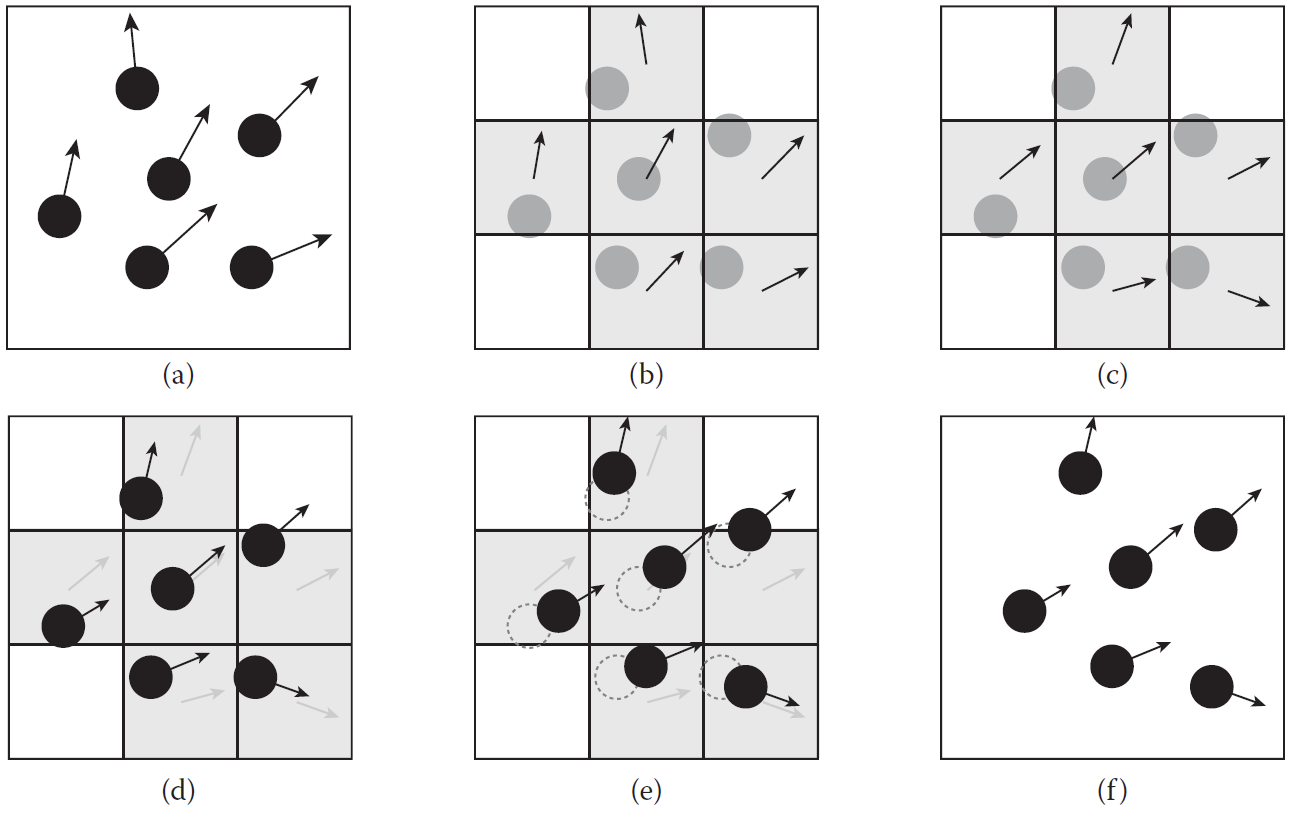
\includegraphics[width=0.55\linewidth]{figures/Pipeline.PNG}
        \caption{Imagem retirada de \textit{Fluid Engine Development}, de Doyub Kim.}
        \label{fig:pipeline}
    \end{figure}
\end{frame}

\begin{frame}{Fundamentos}
    \begin{figure}
        \centering
        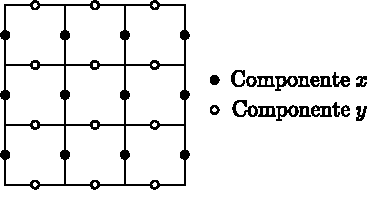
\includegraphics{figures/FaceCenteredGrid.pdf}
        \caption{A velocidade do fluido é armazenada em uma grade regular com pontos nos centros da face.}
        \label{fig:facecenteredgrid}
    \end{figure}
\end{frame}

\begin{frame}{Fundamentos}
    \begin{figure}
        \centering
        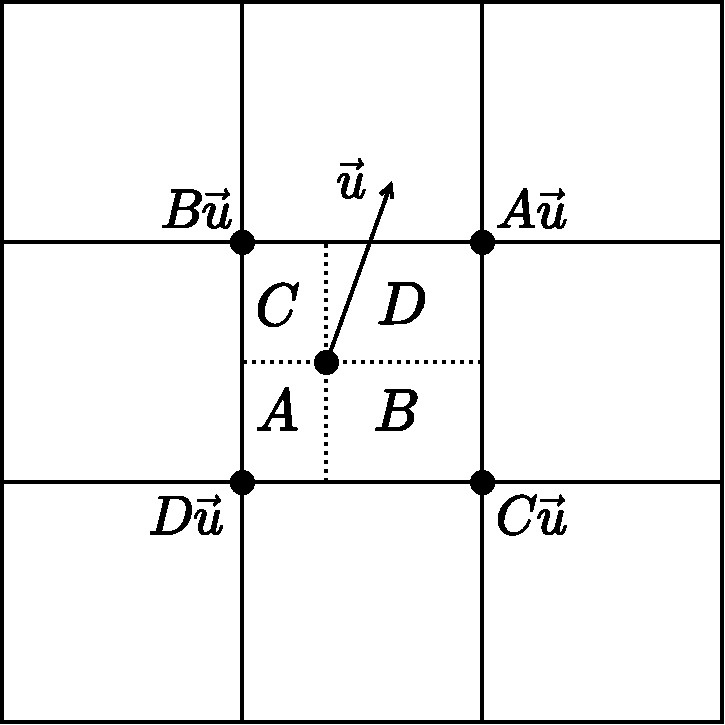
\includegraphics[width=0.4\linewidth]{figures/Particle2Grid.pdf}
        \caption{Transferência de partícula para grade.}
        \label{fig:particle2grid}
    \end{figure}
\end{frame}

\begin{frame}{Fundamentos}
    \begin{itemize}
        \item Porque usar o FLIP?
    \end{itemize}
    \begin{figure}
        \centering
        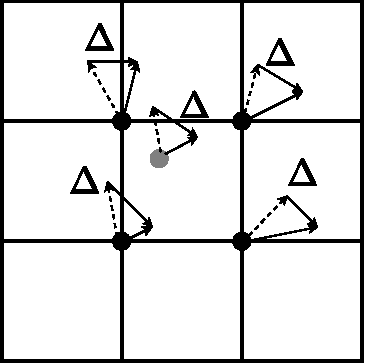
\includegraphics[width=0.4\linewidth]{figures/Grid2Particle.pdf}
        \caption{Transferência da grade para as partículas usada no método FLIP.}
        \label{fig:deltatransfer}
    \end{figure}

\end{frame}

\begin{frame}{Fundamentos}
    
    \only<1>
    {
    \begin{itemize}
        \item Como calcular operadores diferenciais com discretização em grade?
    \end{itemize}
    }
    
    \only<2>
    {
    \begin{itemize}
        \item Diferenças Finitas
    \end{itemize}
    \begin{gather}
        \frac{\partial f}{\partial x} \approx \frac{f^{i+1, j} - f^{i-1,j}}{2\Delta x} \\
        \nabla f \approx \left( \frac{f^{i+1, j} - f^{i-1,j}}{2\Delta x}, \frac{f^{i, j+1} - f^{i,j-1}}{2\Delta y} \right)
    \end{gather}

    \begin{figure}
        \centering
        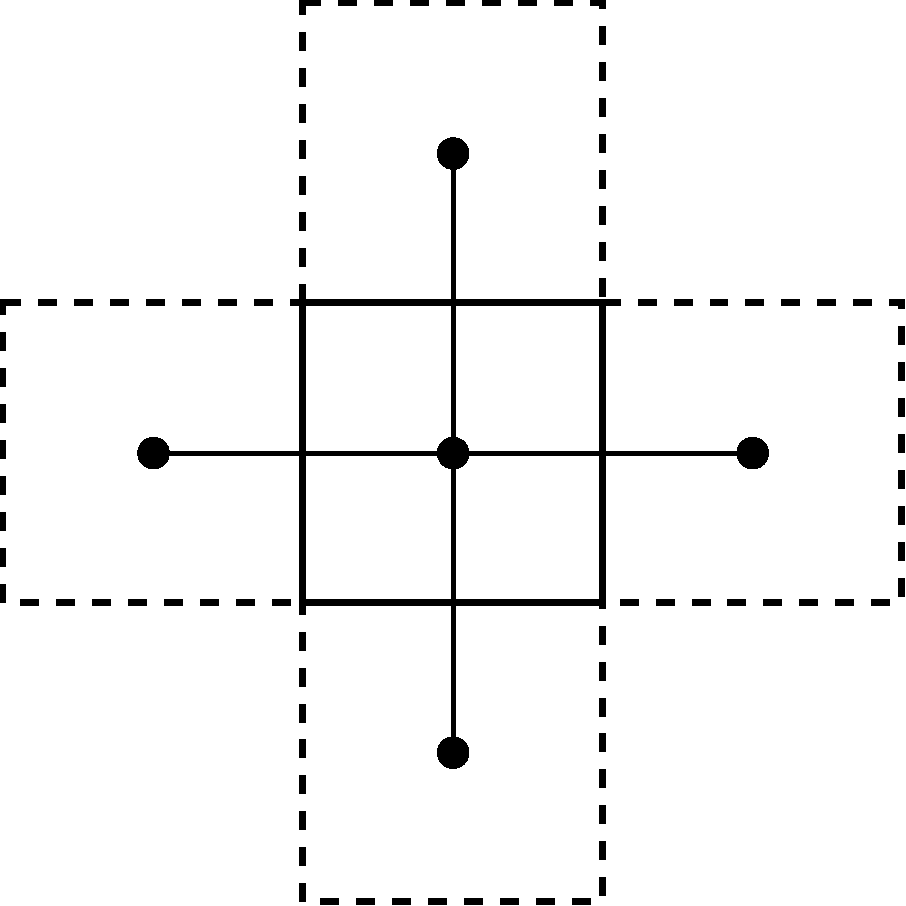
\includegraphics[width=0.20\textwidth]{figures/Stencil.pdf}
        \caption{\textit{Stencil} em uma grade regular.}
        \label{fig:stencil}
    \end{figure}
    }
    
\end{frame}

%-----------------------------------------------

%------------------------------------------------

%------------------------------------------------
\section{Implementação}
%------------------------------------------------

\begin{frame}{Implementação}
    \begin{itemize}
        \item C++ 17
        \item \texttt{CG}
        \item Módulo \texttt{Sparse} de \texttt{Eigen}
        \item Interface gráfica \texttt{ImGui}
    \end{itemize}
\end{frame}

\begin{frame}{Implementação}
    \begin{itemize}
        \item Como solucionar as equações de Navier-Stokes?
    \end{itemize}
\end{frame}

\begin{frame}{Implementação}
\begin{itemize}
    \item Método de Euler implícito para resolver $\mu\nabla^2\Vec{u}$
    \item Resolver sistemas $A \cdot x = b$ para $x$ e $y$
\end{itemize}
\vspace{10px}
    \begin{equation}
        \begin{bmatrix}
            c+1 & -c   &  0 & \cdots & 0 \\
            -c  & 2c+1 & -c & \cdots & 0 \\
            \vdots & \vdots & \ddots & \vdots & \vdots \\
            0 & 0 & \cdots & -c & c+1 \\
        \end{bmatrix}
        \cdot f^{n+1} = f^n,
    \end{equation}
    onde
    \begin{equation}
        c = \frac{\Delta t \mu}{\Delta h^2}.
    \end{equation}
\end{frame}


\begin{frame}{Implementação}
    \begin{figure}
        \centering
        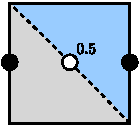
\includegraphics[scale=1.5]{figures/FractionalGrid.pdf}
        \caption{Método fracionário para interface sólido-fluido.}
        \label{fig:fractionalgrid}
    \end{figure}
\end{frame}

\begin{frame}{Implementação}
    Condições de Contorno
    \begin{itemize}
        \item<1-> Solução única para as equações de Navier-Stokes
        \item<2-> Definem o fluxo em interfaces sólidas
    \end{itemize}
    
    \begin{block}<3->{Condição de Contorno de Newmann}
        \begin{equation}
            \Vec{u} \cdot \Vec{n} = 0 
        \end{equation}
    \end{block}
    
    \pause
    
    \begin{block}<4->{Condição de Contorno de Dirichlet}
        \begin{equation}            
            \Vec{u} = \text{max}\left( 1 - \lambda \frac{\text{max}\left(-\Vec{u} \cdot \Vec{n},0\right)}{\lvert \Vec{u}_{p}\rvert}, 0\right) \Vec{u}_{p}
        \end{equation}
    \end{block}
\end{frame}

\begin{frame}{Implementação}
    \begin{itemize}[<+->]
        \item \textit{Signed distance field}
        \item Busca por partículas vizinhas
    \end{itemize}
    
    \only<3->
    {
    \begin{figure}
        \centering
        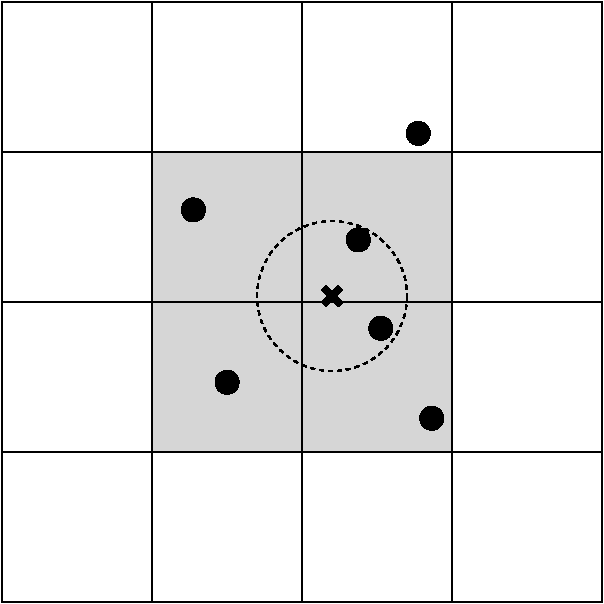
\includegraphics[width=0.3\linewidth]{figures/PointGridHashSearcher.pdf}
        \caption{Busca de partículas vizinhas ao ponto \textbf{x} em um dado raio de busca.}
        \label{fig:gridhashsearcher}
    \end{figure}
    }
\end{frame}

\begin{frame}{Implementação}
    \begin{itemize}
        \item Métricas
        \begin{itemize}
            \item 40 classes
            \item + 5000 linhas de código
        \end{itemize}
    \end{itemize}
    
    \only<1>
    {
    \begin{figure}
        \centering
        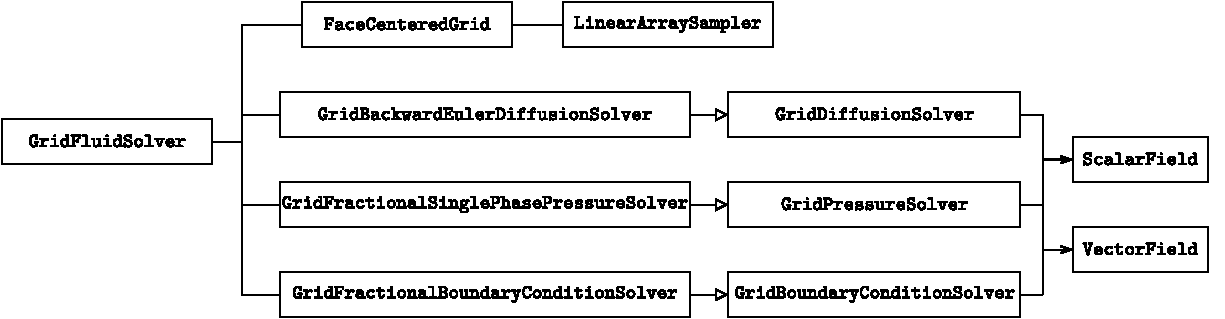
\includegraphics[width=\linewidth]{figures/GridFluidSolveDiagram.pdf}
        \caption{Classe base do solucionador PIC}
        \label{fig:gridfluid}
    \end{figure}
    }
    
    \only<2>
    {
    \begin{figure}
        \centering
        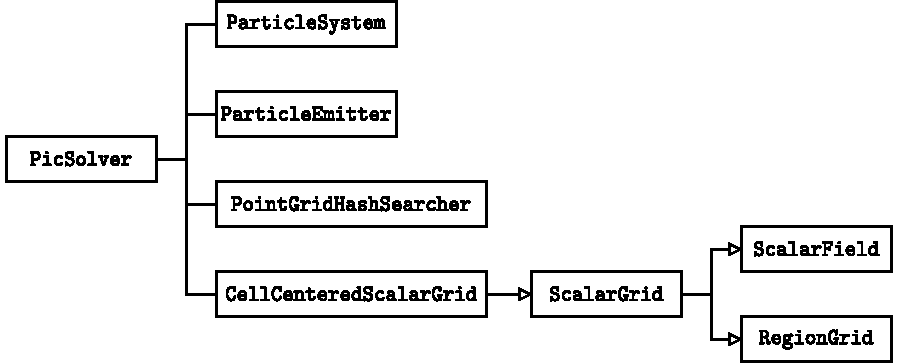
\includegraphics[width=0.8\linewidth]{figures/PicSolver.pdf}
        \caption{Classe base do solucionador FLIP}
        \label{fig:picsolver}
    \end{figure}
    }
\end{frame}

%------------------------------------------------

%------------------------------------------------
\section{Resultados}
%------------------------------------------------

\begin{frame}{Resultados}
    
    \begin{table}[ht]
    \centering
    \begin{tabular}{|l|c|c|c|c|c|}
    \hline
    Cena & \textit{n} & \textit{t} & \textit{F} & $\mu$ & $\rho$ \\ \hline
    DB   & 10500      & 78         & 480        & 0     & 1      \\ \hline
    DB   & 10500      & 91         & 480        & 0.05  & 1      \\ \hline
    DDB  & 22051      & 99         & 480        & 0     & 1      \\ \hline
    WD   & 25073      & 126        & 480        & 0     & 1      \\ \hline
    \end{tabular}
    \caption{Números e parâmetros das simulações.}
    \label{tab:simparams}
    \end{table}
\end{frame}

%------------------------------------------------

\begin{frame}
    \Huge{\centerline{Obrigado!}}
\end{frame}

%----------------------------------------------------------------------------------------

\end{document}